\documentclass[border=15pt]{standalone}
\usepackage{tikz}
\usepackage{amsmath, amssymb}
\usetikzlibrary{calc, arrows.meta, positioning, backgrounds}

% Define a modern, clean UI color palette (Tailwind CSS inspired)
\definecolor{UIBlueMain}{HTML}{2563EB}    % Blue 600
\definecolor{UIBlueLight}{HTML}{EFF6FF}   % Blue 50
\definecolor{UIBlueBorder}{HTML}{BFDBFE}  % Blue 200
\definecolor{UITextDark}{HTML}{1F2937}    % Gray 800
\definecolor{UITextMuted}{HTML}{6B7280}   % Gray 500
\definecolor{UIAccentRose}{HTML}{F43F5E}  % Rose 500

\begin{document}

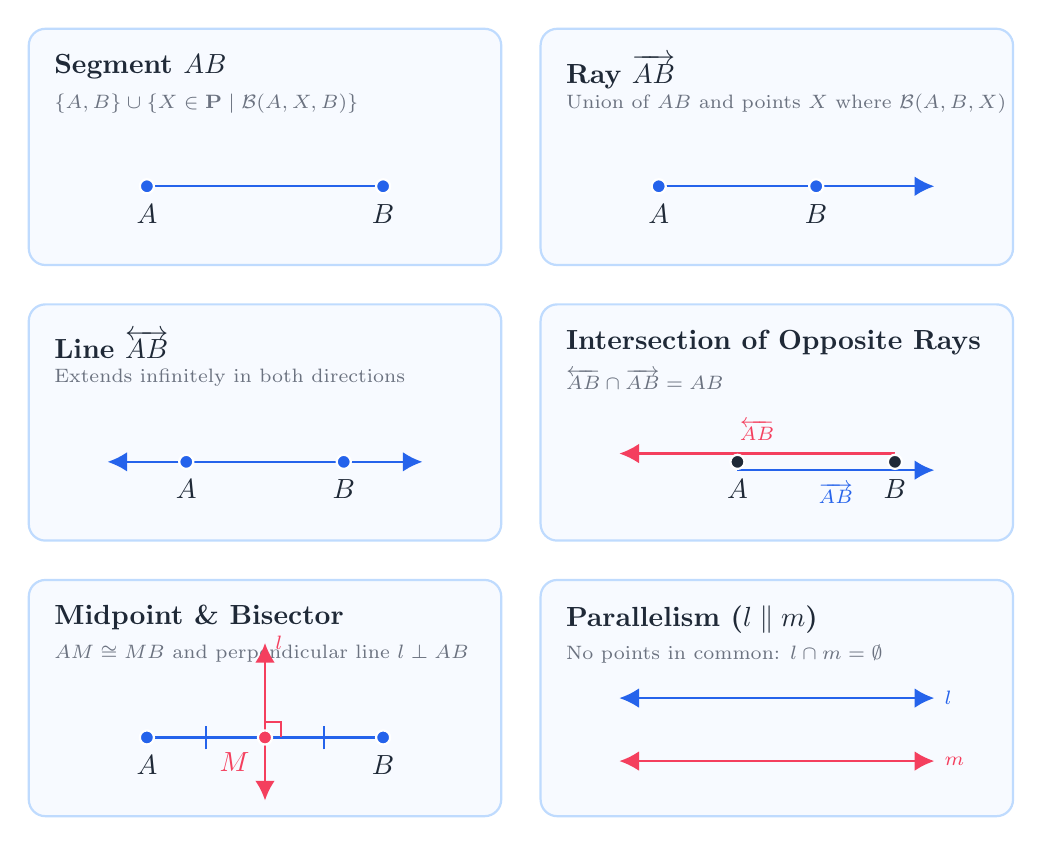
\begin{tikzpicture}[
    font=\sffamily,
    >={Latex[length=2.5mm, width=2.5mm]},
    % UI Component Styles
    panel/.style={fill=UIBlueLight!50, draw=UIBlueBorder, rounded corners=6pt, thick},
    title/.style={font=\bfseries\color{UITextDark}, anchor=north west},
    subtitle/.style={font=\scriptsize\color{UITextMuted}, anchor=north west},
    % Geometry Element Styles
    point/.style={circle, fill=UIBlueMain, draw=white, thick, inner sep=1.8pt},
    line/.style={thick, UIBlueMain},
    accentline/.style={thick, UIAccentRose}
]

    % ==========================================
    % PANEL 1: Segment
    % ==========================================
    \begin{scope}[shift={(0,0)}]
        \filldraw[panel] (0,0) rectangle (6,3);
        \node[title] at (0.2, 2.8) {Segment $AB$};
        \node[subtitle] at (0.2, 2.3) {$\{A, B\} \cup \{X \in \mathbf{P} \mid \mathcal{B}(A, X, B)\}$};

        \coordinate (A) at (1.5, 1);
        \coordinate (B) at (4.5, 1);

        \draw[line] (A) -- (B);
        \node[point, label={[UITextDark]below:{$A$}}] at (A) {};
        \node[point, label={[UITextDark]below:{$B$}}] at (B) {};
    \end{scope}

    % ==========================================
    % PANEL 2: Ray
    % ==========================================
    \begin{scope}[shift={(6.5,0)}]
        \filldraw[panel] (0,0) rectangle (6,3);
        \node[title] at (0.2, 2.8) {Ray $\overrightarrow{AB}$};
        \node[subtitle] at (0.2, 2.3) {Union of $AB$ and points $X$ where $\mathcal{B}(A, B, X)$};

        \coordinate (A) at (1.5, 1);
        \coordinate (B) at (3.5, 1);
        \coordinate (End) at (5, 1);

        \draw[line, ->] (A) -- (End);
        \node[point, label={[UITextDark]below:{$A$}}] at (A) {};
        \node[point, label={[UITextDark]below:{$B$}}] at (B) {};
    \end{scope}

    % ==========================================
    % PANEL 3: Line
    % ==========================================
    \begin{scope}[shift={(0,-3.5)}]
        \filldraw[panel] (0,0) rectangle (6,3);
        \node[title] at (0.2, 2.8) {Line $\overleftrightarrow{AB}$};
        \node[subtitle] at (0.2, 2.3) {Extends infinitely in both directions};

        \coordinate (Start) at (1, 1);
        \coordinate (A) at (2, 1);
        \coordinate (B) at (4, 1);
        \coordinate (End) at (5, 1);

        \draw[line, <->] (Start) -- (End);
        \node[point, label={[UITextDark]below:{$A$}}] at (A) {};
        \node[point, label={[UITextDark]below:{$B$}}] at (B) {};
    \end{scope}

    % ==========================================
    % PANEL 4: Opposite Rays (Intersection)
    % ==========================================
    \begin{scope}[shift={(6.5,-3.5)}]
        \filldraw[panel] (0,0) rectangle (6,3);
        \node[title] at (0.2, 2.8) {Intersection of Opposite Rays};
        \node[subtitle] at (0.2, 2.3) {$\overleftarrow{AB} \cap \overrightarrow{AB} = AB$};

        \coordinate (Start) at (1, 1);
        \coordinate (A) at (2.5, 1);
        \coordinate (B) at (4.5, 1);
        \coordinate (End) at (5, 1);

        % Ray BA (shifted slightly up)
        \draw[accentline, <-, transform canvas={yshift=3pt}]
            (Start) -- (B) node[midway, above=1pt, font=\scriptsize, UIAccentRose] {$\overleftarrow{AB}$};

        % Ray AB (shifted slightly down)
        \draw[line, ->, transform canvas={yshift=-3pt}]
            (A) -- (End) node[midway, below=1pt, font=\scriptsize, UIBlueMain] {$\overrightarrow{AB}$};

        \node[point, fill=UITextDark, label={[UITextDark]below:{$A$}}] at (A) {};
        \node[point, fill=UITextDark, label={[UITextDark]below:{$B$}}] at (B) {};
    \end{scope}

    % ==========================================
    % PANEL 5: Midpoint & Bisector
    % ==========================================
    \begin{scope}[shift={(0,-7)}]
        \filldraw[panel] (0,0) rectangle (6,3);
        \node[title] at (0.2, 2.8) {Midpoint \& Bisector};
        \node[subtitle] at (0.2, 2.3) {$AM \cong MB$ and perpendicular line $l \perp AB$};

        \coordinate (A) at (1.5, 1);
        \coordinate (B) at (4.5, 1);
        \coordinate (M) at (3, 1);
        \coordinate (T) at (3, 2.2);
        \coordinate (Bot) at (3, 0.2);

        \draw[line] (A) -- (B);
        \draw[accentline, <->] (Bot) -- (T) node[right, font=\scriptsize, UIAccentRose] {$l$};

        % Right angle marker
        \draw[accentline] (3, 1.2) -- (3.2, 1.2) -- (3.2, 1);

        % Congruence Tick marks
        \draw[line] (2.25, 0.85) -- (2.25, 1.15);
        \draw[line] (3.75, 0.85) -- (3.75, 1.15);

        \node[point, label={[UITextDark]below:{$A$}}] at (A) {};
        \node[point, label={[UITextDark]below:{$B$}}] at (B) {};
        \node[point, fill=UIAccentRose, label={[UIAccentRose]below left:{$M$}}] at (M) {};
    \end{scope}

    % ==========================================
    % PANEL 6: Parallelism
    % ==========================================
    \begin{scope}[shift={(6.5,-7)}]
        \filldraw[panel] (0,0) rectangle (6,3);
        \node[title] at (0.2, 2.8) {Parallelism ($l \parallel m$)};
        \node[subtitle] at (0.2, 2.3) {No points in common: $l \cap m = \emptyset$};

        \coordinate (L1) at (1, 1.5);
        \coordinate (R1) at (5, 1.5);
        \coordinate (L2) at (1, 0.7);
        \coordinate (R2) at (5, 0.7);

        \draw[line, <->] (L1) -- (R1) node[right, font=\scriptsize\bfseries, UIBlueMain] {$l$};
        \draw[accentline, <->] (L2) -- (R2) node[right, font=\scriptsize\bfseries, UIAccentRose] {$m$};
    \end{scope}

\end{tikzpicture}

\end{document}
